\documentclass[final]{article}
\PassOptionsToPackage{numbers,sort&compress}{natbib}

\usepackage{aps360}
\usepackage[utf8]{inputenc} % allow utf-8 input
\usepackage[T1]{fontenc}    % use 8-bit T1 fonts
\usepackage{hyperref}       % hyperlinks
\usepackage{url}            % simple URL typesetting
\usepackage{booktabs}       % professional-quality tables
\usepackage{amsfonts,amsmath,amssymb}
\usepackage{nicefrac}       % compact symbols for 1/2, etc.
\usepackage{microtype}      % microtypography
\usepackage{xcolor}         % colors
\usepackage{graphicx}       % figures
\usepackage{tikz}
\usetikzlibrary{positioning,arrows.meta,fit}
\usepackage{enumitem}
\usepackage[font=small,skip=3pt]{caption}
\setlist{nosep,leftmargin=*}
\graphicspath{{../figures/}{./}} % figures written by the scripts in src/

% ---------------------------------------------------------------- results
% The scripts write LaTeX macros with every number used below:
%   src/training/train.py            figures/results_macros.tex   (\AnnValAcc, \CnnHasyFtAcc, ...)
%   src/data_collection/hasy.py      figures/hasy_macros.tex
% A number whose file does not exist yet shows as a red [TBD].
\newcommand{\TBD}[1][]{\textcolor{red}{[TBD#1]}}
\newcommand{\inputif}[1]{\IfFileExists{../figures/#1.tex}{\input{../figures/#1.tex}}{}}
\inputif{results_macros}\inputif{hasy_macros}
\newcommand{\res}[1]{\ifcsname #1\endcsname\csname #1\endcsname\else\TBD\fi}
\newcommand{\maybefig}[2]{\IfFileExists{../figures/#2.pdf}{\includegraphics[#1]{#2}}%
  {\fbox{\parbox[c][2cm][c]{0.9\linewidth}{\centering\TBD[: \texttt{\detokenize{#2}}]}}}}
\newcommand{\cmd}[1]{\texttt{\textbackslash #1}}

\title{From Pixels to \LaTeX: Classifying Math Symbol\\Images into \LaTeX{} Commands {\large(Progress Report)}}

\author{%
  Alan Wang \\
  1011974874, alanwyt.wang@mail.utoronto.ca\\
  Code: \url{https://github.com/yutong-wang-7/aps360-pixels-to-latex}\\
}

\begin{document}

\maketitle

\vspace{-0.45in}

% =====================================================================
\section{Brief Project Description}
\vspace{-0.05in}

Writing math in \LaTeX{} is slowed down by recall: I recognize a symbol but forget its command
(\cmd{epsilon} or \cmd{varepsilon}? \cmd{propto}?). Detexify~\cite{detexify} solves this for symbols
drawn with a mouse; my goal is the image version, a lookup tool for students and researchers who
recognize a symbol but not its command. \textbf{Input:} a $32{\times}32$ image of one math symbol;
\textbf{output:} its \LaTeX{} command, one of $K=160$ classes (digits, Latin and Greek letters, operators,
relations, arrows, delimiters; Fig.~\ref{fig:pipeline}). The same classifier is also tested on handwritten
symbols. Deep learning fits because there is no single template per class: a symbol's shape varies with
font, stroke weight and handwriting style (Fig.~\ref{fig:data}), many classes are near-identical
($\epsilon/\varepsilon$, $\phi/\varphi$, ${\cdot}/.$, $l/I/|$), and a CNN learns local stroke features
that tolerate small shifts. Rendered training labels are free and unlimited, and success is measured only
on fonts and writers never seen in training.

\begin{figure}[h]
\centering
\begin{tikzpicture}[
  font=\scriptsize, >={Stealth[length=4pt]}, node distance=2mm,
  b/.style={draw, rounded corners=1pt, align=center, minimum height=7.5mm, inner sep=2pt},
  conv/.style={b, fill=blue!18, font=\tiny}, fc/.style={b, fill=teal!18}, outn/.style={b, fill=green!15}]
  \node (in) {
\includegraphics[width=11mm]{fig_input.png}};
  \node[below=0mm of in, align=center] {input $1{\times}32{\times}32$\\(\cmd{varphi}, val font)};
  % CNN row
  \node[conv, right=6mm of in, yshift=6mm] (c1) {Conv $3{\times}3$, BN,\\ReLU, MaxPool\\$32{\times}16{\times}16$};
  \node[conv, right=of c1] (c2) {Conv $3{\times}3$, BN,\\ReLU, MaxPool\\$64{\times}8{\times}8$};
  \node[conv, right=of c2] (c3) {Conv $3{\times}3$, BN,\\ReLU, MaxPool\\$128{\times}4{\times}4$};
  \node[conv, right=of c3] (c4) {Conv $3{\times}3$, BN,\\ReLU, MaxPool\\$256{\times}2{\times}2$};
  \node[fc, right=of c4] (f1) {Flatten 1024\\FC 256, ReLU\\Dropout 0.3};
  \node[fc, right=of f1] (f2) {FC 160};
  % ANN row
  \node[fc, right=6mm of in, yshift=-8mm] (a0) {Flatten\\1024};
  \node[fc, right=of a0] (a1) {FC 256, ReLU\\Dropout 0.3};
  \node[fc, right=of a1] (a2) {FC 128, ReLU\\Dropout 0.3};
  \node[fc] (a3) at (a2 -| f2) {FC 160};
  \node[outn, right=6mm of f2, yshift=-7mm] (o) {softmax\\$\arg\max$\\\cmd{varphi}};
  \draw[->] (in.east) -- ++(2mm,0) |- (c1.west);
  \draw[->] (in.east) -- ++(2mm,0) |- (a0.west);
  \foreach \u/\v in {c1/c2,c2/c3,c3/c4,c4/f1,f1/f2,a0/a1,a1/a2,a2/a3} \draw[->] (\u) -- (\v);
  \draw[->] (f2.east) -- ++(2mm,0) |- (o.west);
  \draw[->] (a3.east) -- ++(2mm,0) |- (o.west);
  \node[anchor=south west, text=blue!60!black] at (c1.north west) {\textbf{Primary CNN} (\res{CnnParams} parameters)};
  \node[anchor=north west, text=teal!50!black] at (a0.south west) {\textbf{Baseline ANN} (\res{AnnParams} parameters)};
\end{tikzpicture}
\caption{Input, output, and the two models (same data, loss and training loop; 160-way output).}
\label{fig:pipeline}
\end{figure}
\vspace{-0.15in}

% =====================================================================
\section{Notable Contribution}
\vspace{-0.05in}

\subsection{Data Processing}
\vspace{-0.05in}

I use two datasets (Table~\ref{tab:data}). All processing is scripted and seeded
(\texttt{src/data\_collection/}, about 2 minutes on a CPU).

\begin{table}[h]
\centering\small
\caption{Datasets. Train / validation / test never share a font family (printed) or a writer
(handwritten). Printed: clean renders (+ augmented copies); val / test also have augmented copies, used only as a robustness check.}
\label{tab:data}
\setlength{\tabcolsep}{4pt}\footnotesize
\begin{tabular}{llll}
\toprule
Data (source) & Train & Val & Test \\
\midrule
Printed symbols (18 fonts~\cite{ctan}) & 11 fonts: 2{,}768 + 102{,}712 aug. & 3 fonts: 756 & 4 fonts: 1{,}007 \\
Handwritten (HASYv2~\cite{hasy}) & \res{HasySplitTrainImages} & \res{HasySplitValImages} (\res{HasySplitValWriters} writers) & \res{HasySplitTestImages} (\res{HasySplitTestWriters} writers) \\
\bottomrule
\end{tabular}
\end{table}

\textbf{Printed symbols} (\texttt{make\_dataset.py}). Each class stores its \LaTeX{} label and the
Unicode code points of its upright and math-italic forms.
\begin{enumerate}
  \item \textbf{Render and normalize.} A (class, style, font) is kept only if the font has the glyph and
  the render has $\geq$20 ink pixels (3 of 2{,}880 class--font pairs are missing). Glyphs are rendered at
  a 128\,px em, cropped to the ink box, padded to a square, and area-resized so the longest side is
  28\,px in a $32{\times}32$ canvas (ink $=255$). Letters are math italic 70\% of the time, upright 30\%.
  \item \textbf{Augmentation} (60 images per class and training font, clean renders included; Fig.~\ref{fig:data}). Rotation
  $\pm8^\circ$, size 22--30\,px, shift $\pm2$\,px, stroke weight, blur, noise, plus four
  handwriting-style steps: elastic warp, slant (shear $\pm0.3$), binarization, and a \emph{pen} redraw
  (binarize, thin to a 1\,px skeleton with Zhang--Suen thinning, redraw at 1--3\,px).
  \item \textbf{Split by font family.} I measured font similarity as the mean normalized pixel difference
  over all classes; the build stops if two fonts in different splits are closer than 0.34
  (same family: 0.02--0.36; closest cross-split pair: 0.359). Classes whose renders are near-identical in every font would be merged; none are.
\end{enumerate}
\textbf{Handwritten symbols} (\texttt{hasy.py}). HASYv2 labels are mapped to mine (exact match plus
aliases such as \cmd{le}$\to$\cmd{leq}) and the images get the same crop--pad--resize step. HASY's official
folds share writers across folds, and one user id holds 76k of the 87k mapped images with no known writer,
no images at all of 24 classes, and a skewed class mix. So I split \emph{identified} writers as whole
writers (about 50/25/25\% of their images to train/val/test) and put the bulk id in train.

\textbf{Class balance.} Printed classes are balanced: 600--660 training images and 3--6 clean validation
images per class. HASY's training images are not (20 to 2{,}877 per class; \cmd{infty} is the most
common), so fine-tuning samples classes uniformly; its validation writers are more even (no class above 2\%).


\begin{figure}[h]
\centering
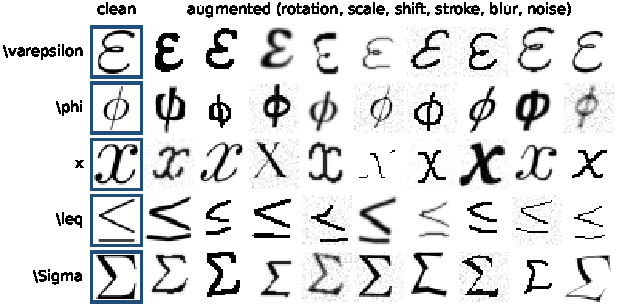
\includegraphics[width=0.5\linewidth]{fig_augmented}
\caption{Clean training renders (boxed) and augmented copies.}
\label{fig:data}
\end{figure}
\vspace{-0.1in}

\textbf{Testing on never-seen data.} Model choices use only validation data. For the final report I will
evaluate once on (1)~the 4 test fonts, never used for training or model selection, and (2)~the HASY test
writers (handwritten), who appear in no other split.

\textbf{Challenges.} Anti-aliasing makes exact pixel-identity checks for identical classes impossible, so I
use a tolerance. Erewhon (Utopia) is 0.34 from STIX~Two, as close as fonts within one family, so I kept
both in training. At first, HASY's bulk user id left 16\% of the handwritten validation images in classes
with no handwritten training data; the writer split above fixed this. Printed strokes are thick with varying contrast, while
pen strokes are thin and even, which motivated the pen redraw.

% =====================================================================
\subsection{Baseline Model: ANN}
\vspace{-0.05in}

My baseline is the ANN from my proposal: the flattened image passes through FC layers
$1024{\to}256{\to}128{\to}160$ with ReLU and dropout 0.3 (\res{AnnParams} parameters). It is easy to
implement and has no spatial inductive bias, so the gap to the CNN shows what convolution adds.
\textbf{Shared setup} (PyTorch~\cite{pytorch}, \texttt{src/training/}): cross-entropy, Adam (weight decay
$10^{-4}$), 12 epochs with a cosine schedule, keeping the epoch with the best clean-validation
accuracy; every source of randomness is seeded (360). Learning rate, batch size and model size come from a
grid search (6 epochs on 30\% of the training images; 16 ANN and 96 CNN settings, Table~\ref{tab:tune} in
the appendix), scored by the mean of the printed and handwritten validation errors. The ANN uses width
256, learning rate $3{\times}10^{-3}$ and batch 256.

\textbf{Results} (Table~\ref{tab:res}). On the unseen validation fonts the ANN reaches \res{AnnValAcc}\%
top-1 (macro-F1 \res{AnnValFOne}\%), but only \res{AnnValAugAcc}\% on their augmented copies and
\res{AnnHasyZeroAcc}\% on handwriting. \textbf{Qualitative.} The ANN is brittle to small geometric changes: a 2\,px
shift moves every input pixel, so it loses about 11 points on the augmented copies, against about 4 for the
CNN. \textbf{Challenges.} The ANN underfits the augmented training data: its training accuracy is only
\res{AnnTrainAcc}\%, below its clean validation accuracy, while the CNN reaches \res{CnnTrainAcc}\%.

% =====================================================================
\subsection{Primary Model: CNN}
\vspace{-0.05in}

\textbf{Architecture} (Fig.~\ref{fig:pipeline}). Four blocks of $3{\times}3$ convolution (padding 1),
batch normalization, ReLU and $2{\times}2$ max pooling; channels $1{\to}32{\to}64{\to}128{\to}256$ while the
image shrinks $32{\to}16{\to}8{\to}4{\to}2$; then flatten (1024), FC~256 (ReLU, dropout 0.3) and FC~160: 6
weight layers, \res{CnnParams} parameters (38\% in the first FC layer). Among 2--4 blocks, width 16/32 and
FC 128/256, the grid search chose 4 blocks, width 32, learning rate $10^{-3}$ and batch 64: printed
accuracy was similar across the top settings, and this one had the best handwriting accuracy. Training takes
\res{CnnTrainMin} minutes on \res{Device} (fine-tuning about 3 more); the full training script, including
evaluation, takes about 10 minutes, and the 96-setting CNN grid search about 26. \textbf{Fine-tuning for handwriting.} Starting from the printed
model, all layers keep training (learning rate $3{\times}10^{-4}$, up to 16 epochs) on printed plus HASY
training images, with class-balanced batches (half printed, half handwritten, classes equally likely), and
the epoch is selected on the HASY validation writers.

\begin{table}[h]
\centering\small
\caption{Validation results (\%), all on fonts / writers never used in training. Merged:
a prediction in the true class's near-identical group counts as correct (12 groups, e.g.\ $o/O/0/\circ$;
appendix).}
\label{tab:res}
\setlength{\tabcolsep}{4pt}
\begin{tabular}{lrrrrrr}
\toprule
& \multicolumn{3}{c}{Printed symbols} & \multicolumn{3}{c}{Handwritten symbols} \\
\cmidrule(lr){2-4}\cmidrule(lr){5-7}
Model & Acc & Merged & Aug. & Zero-shot & Fine-tuned & Merged \\
\midrule
ANN & \res{AnnValAcc} & \res{AnnValAccMerged} & \res{AnnValAugAcc} & \res{AnnHasyZeroAcc} & \res{AnnHasyFtAcc} & \res{AnnHasyFtAccMerged} \\
CNN & \textbf{\res{CnnValAcc}} & \textbf{\res{CnnValAccMerged}} & \textbf{\res{CnnValAugAcc}} & \textbf{\res{CnnHasyZeroAcc}} & \textbf{\res{CnnHasyFtAcc}} & \textbf{\res{CnnHasyFtAccMerged}} \\
\bottomrule
\end{tabular}
\end{table}

\textbf{Results.} The CNN beats the ANN on every metric (Table~\ref{tab:res}, Fig.~\ref{fig:curves}). On
printed symbols both are near the ceiling (\res{CnnValAcc} vs.\ \res{AnnValAcc}\%; top-5 is
\res{CnnValTopFive}\%), so the gap shows most under distortion (augmented copies) and handwriting:
\res{CnnHasyZeroAcc}\% zero-shot vs.\ \res{AnnHasyZeroAcc}\%, and \res{CnnHasyFtAcc}\% after fine-tuning
(\res{CnnHasyFtAccMerged}\% merged), while printed accuracy stays at \res{CnnHasyFtPrintedAcc}\%. Macro-F1 is within 2 points of accuracy
(printed \res{CnnValFOne} vs.\ \res{CnnValAcc}\%; handwriting 76.4 vs.\ 78.4\%), so the accuracy is not
driven by a few frequent classes.
\textbf{Qualitative.} Most printed errors are look-alike pairs. For $s\to S$ (19 of 36 clean and
augmented validation images; 32 for the ANN), ${\cdot}\leftrightarrow.$ and $c\to C$, size is the only cue
left after cropping; $Y/\Upsilon$ is a similar pair that is not merged (Table~\ref{tab:conf}). On
handwriting, 31\% of the fine-tuned CNN's errors fall inside a near-identical group ($s\to S$,
$v\to\vee$, $o\to\circ$); the most frequent other errors are $\pi\to\Pi$, $\alpha\to\propto$, $U\to\cup$
and $g\to9$, which writers often draw alike (Table~\ref{tab:hconf}; samples in Fig.~\ref{fig:hasy}).
\textbf{Challenges.} The validation fonts are all Palatino-like and easy, so they barely separate the models;
I therefore also use handwriting accuracy when tuning. Before the writer split and class-balanced batches,
fine-tuning stalled at 56.5\% because 24 classes had no handwritten training images.

\begin{figure}[h]
\centering
\maybefig{width=0.72\linewidth}{fig_curves}
\caption{Learning curves. Dashed: training images (augmented); solid: clean validation images (unseen fonts).}
\label{fig:curves}
\end{figure}
\vspace{-0.1in}

\textbf{Feasibility and plan.} I am on track: all data is generated and split, both models are trained and
evaluated on validation data, and the whole pipeline (generation, tuning, training, evaluation) is
scripted. A full run takes about 10 minutes on my GPU, so the remaining time can go to improvements and
analysis. Remaining work: (1)~improve handwriting accuracy (\res{CnnHasyFtAcc}\% vs.\ \res{CnnValAcc}\% on
printed), e.g.\ with ensembles of CNNs; (2)~possibly compare a small Vision Transformer once it is covered
in the course; (3)~evaluate once on the test fonts and test writers; (4)~stretch goal for the final report,
flat printed equations: render generated equations with symbol boxes, split them into symbols with
connected components, classify each crop with the CNN, and report exact match with segmentation and
classification errors counted separately.

\newpage
\begin{thebibliography}{9}\small
\bibitem{detexify} D.~Kirsch. Detexify \LaTeX{} handwritten symbol recognition. \url{https://detexify.kirelabs.org}. Accessed Nov.~2026.
\bibitem{ctan} The Comprehensive \TeX{} Archive Network (CTAN): \texttt{lm-math}, \texttt{newcomputermodern}, \texttt{tex-gyre-math}, \texttt{stix2-otf}, \texttt{xits}, \texttt{libertinus-fonts}, \texttt{garamond-math}, \texttt{euler-math}, \texttt{erewhon-math}, \texttt{kpfonts-otf}, \texttt{Asana-Math}, \texttt{concmath-otf}, \texttt{lete-sans-math}, \texttt{firamath}. \url{https://ctan.org}. Accessed Nov.~2026.
\bibitem{hasy} M.~Thoma. The HASYv2 dataset. arXiv:1701.08380, 2017.
\bibitem{pytorch} A.~Paszke et al. PyTorch: An imperative style, high-performance deep learning library. In \emph{NeurIPS}, 2019.
\end{thebibliography}

% =====================================================================
\appendix
\section{Appendix}

\textbf{Near-identical groups} (used only for the ``merged'' metrics; rule: same shape up to size or
position once cropped to the ink box, plus the look-alikes named in my proposal):
{\small\inputif{near_identical}}

\begin{table}[h]
\centering\small
\begin{minipage}[t]{0.44\linewidth}
  \centering
  \captionof{table}{Most frequent CNN confusions on the printed validation fonts, clean plus augmented
  images (count / images of the true class), with the ANN's count for the same pair.}
  \label{tab:conf}
  \IfFileExists{../figures/confusions_table.tex}{\begin{tabular}{llrr}
\toprule
True & Predicted & CNN & ANN \\
\midrule
\texttt{s} & \texttt{S} & 19/36 & 32/36 \\
\texttt{\textbackslash{}cdot} & \texttt{.} & 17/33 & 13/33 \\
\texttt{.} & \texttt{\textbackslash{}cdot} & 13/33 & 14/33 \\
\texttt{Y} & \texttt{\textbackslash{}Upsilon} & 12/36 & 2/36 \\
\texttt{c} & \texttt{C} & 10/36 & 6/36 \\
\texttt{\textbackslash{}Upsilon} & \texttt{Y} & 10/36 & 11/36 \\
\texttt{\textbackslash{}upsilon} & \texttt{v} & 8/36 & 3/36 \\
\texttt{,} & \texttt{/} & 8/33 & 4/33 \\
\bottomrule
\end{tabular}
}{\TBD}
\end{minipage}\hfill
\begin{minipage}[t]{0.52\linewidth}
  \centering
  \captionof{table}{Most frequent errors of the fine-tuned CNN on the handwritten validation writers.
  Merged: both classes are in one near-identical group.}
  \label{tab:hconf}
  \IfFileExists{../figures/hasy_confusions_table.tex}{% CNN ft on HASY val writers: 591 errors, 186 inside near-identical groups
\begin{tabular}{llrc}
\toprule
True & Predicted & Count & Merged \\
\midrule
\texttt{s} & \texttt{S} & 15/20 & yes \\
\texttt{v} & \texttt{\textbackslash{}vee} & 14/16 & yes \\
\texttt{o} & \texttt{\textbackslash{}circ} & 13/22 & yes \\
\texttt{V} & \texttt{\textbackslash{}vee} & 10/12 & yes \\
\texttt{\textbackslash{}pi} & \texttt{\textbackslash{}Pi} & 10/25 &  \\
\texttt{\textbackslash{}alpha} & \texttt{\textbackslash{}propto} & 10/49 &  \\
\texttt{U} & \texttt{\textbackslash{}cup} & 9/15 &  \\
\texttt{0} & \texttt{\textbackslash{}circ} & 9/30 & yes \\
\texttt{x} & \texttt{\textbackslash{}times} & 9/20 & yes \\
\texttt{z} & \texttt{Z} & 9/20 & yes \\
\texttt{I} & \texttt{|} & 8/24 & yes \\
\texttt{p} & \texttt{P} & 8/18 &  \\
\texttt{g} & \texttt{9} & 7/18 &  \\
\texttt{w} & \texttt{W} & 7/20 & yes \\
\texttt{O} & \texttt{\textbackslash{}circ} & 7/17 & yes \\
\bottomrule
\end{tabular}
}{\TBD}
\end{minipage}
\end{table}

\begin{table}[h]
\centering\small
\caption{Hyperparameter search, best 5 settings per model (6 epochs on 30\% of the training images). Val
acc: printed validation fonts; Hand.: handwritten validation writers (zero-shot). Selected setting (lowest
mean error) in bold.}
\label{tab:tune}
\resizebox{\linewidth}{!}{\IfFileExists{../figures/tuning_table.tex}{\begin{tabular}{llrrrr}
\toprule
Model & Setting & Params & Best epoch & Val acc & Hand. val acc \\
\midrule
ANN (baseline), best 5 of 16 & lr 0.003, bs 256, hidden 256 & 316k & 6 & \textbf{93.1} & \textbf{41.6} \\
 & lr 0.001, bs 64, hidden 256 & 316k & 6 & 93.1 & 41.5 \\
 & lr 0.003, bs 64, hidden 256 & 316k & 6 & 91.4 & 42.0 \\
 & lr 0.001, bs 256, hidden 256 & 316k & 6 & 90.1 & 40.4 \\
 & lr 0.003, bs 256, hidden 128 & 168k & 6 & 90.3 & 39.0 \\
\midrule
CNN (primary), best 5 of 96 & lr 0.001, bs 64, layers 4, ch 32, hidden 256 & 692k & 6 & \textbf{97.0} & \textbf{62.9} \\
 & lr 0.001, bs 64, layers 3, ch 32, hidden 256 & 659k & 6 & 97.8 & 61.0 \\
 & lr 0.001, bs 256, layers 4, ch 32, hidden 256 & 692k & 6 & 96.0 & 62.6 \\
 & lr 0.001, bs 64, layers 4, ch 16, hidden 256 & 270k & 4 & 97.1 & 61.4 \\
 & lr 0.0003, bs 64, layers 4, ch 32, hidden 128 & 541k & 4 & 97.0 & 60.5 \\
\bottomrule
\end{tabular}
}{\TBD}}
\end{table}

\textbf{AI usage.} I used Claude (Anthropic) as a coding and writing assistant. It helped implement
parts of the code, in particular the data generation (font rendering, augmentation, HASYv2 conversion),
the evaluation and plotting helpers, and it wrote most of the code comments; it also helped edit this
report. The model and training-loop code (\texttt{models.py}, \texttt{train\_loop.py}: \texttt{train\_net},
\texttt{evaluate}, \texttt{get\_model\_name}, \texttt{plot\_training\_curve}) follows the APS360 lab
templates (Lab~3). I chose the project, the classes, the data splits and the experiments, and I ran and
checked every result reported here.

\begin{figure}[h]
\centering
\maybefig{width=\linewidth}{fig_hasy}
\caption{Random handwritten validation images with each model's prediction (green: correct; ``ft'':
fine-tuned).}
\label{fig:hasy}
\end{figure}

\end{document}
